
\documentclass[ms.tex]{subfiles}
\begin{document}

\section{Introduction}
\label{sec:intro}

From a nucleosynthesis perspective, N is a unique element.
Along with C and He, it is one of only three elements lighter
than iron peak nuclei who owe a significant portion of their abundances to
asymptotic giant branch (AGB) stars~\citep{Johnson2019}.
N is also the primary by-product of the CNO cycle, a cyclic nuclear reaction
which catalyses the conversion of H into He in non-zero metallicity
stars more massive than the sun.
Furthermore, N is among a select group of elements whose spectroscopically
derived abundances do not reflect the birth abundances of evolved stars, a
consequence of internal mixing processes carrying CNO processed material
to the photosphere (see discussion in, e.g.,~\citealp{Vincenzo2021} and
in~\S~\ref{sec:results:vincenzo_comp} below).

\begin{figure*}
\centering
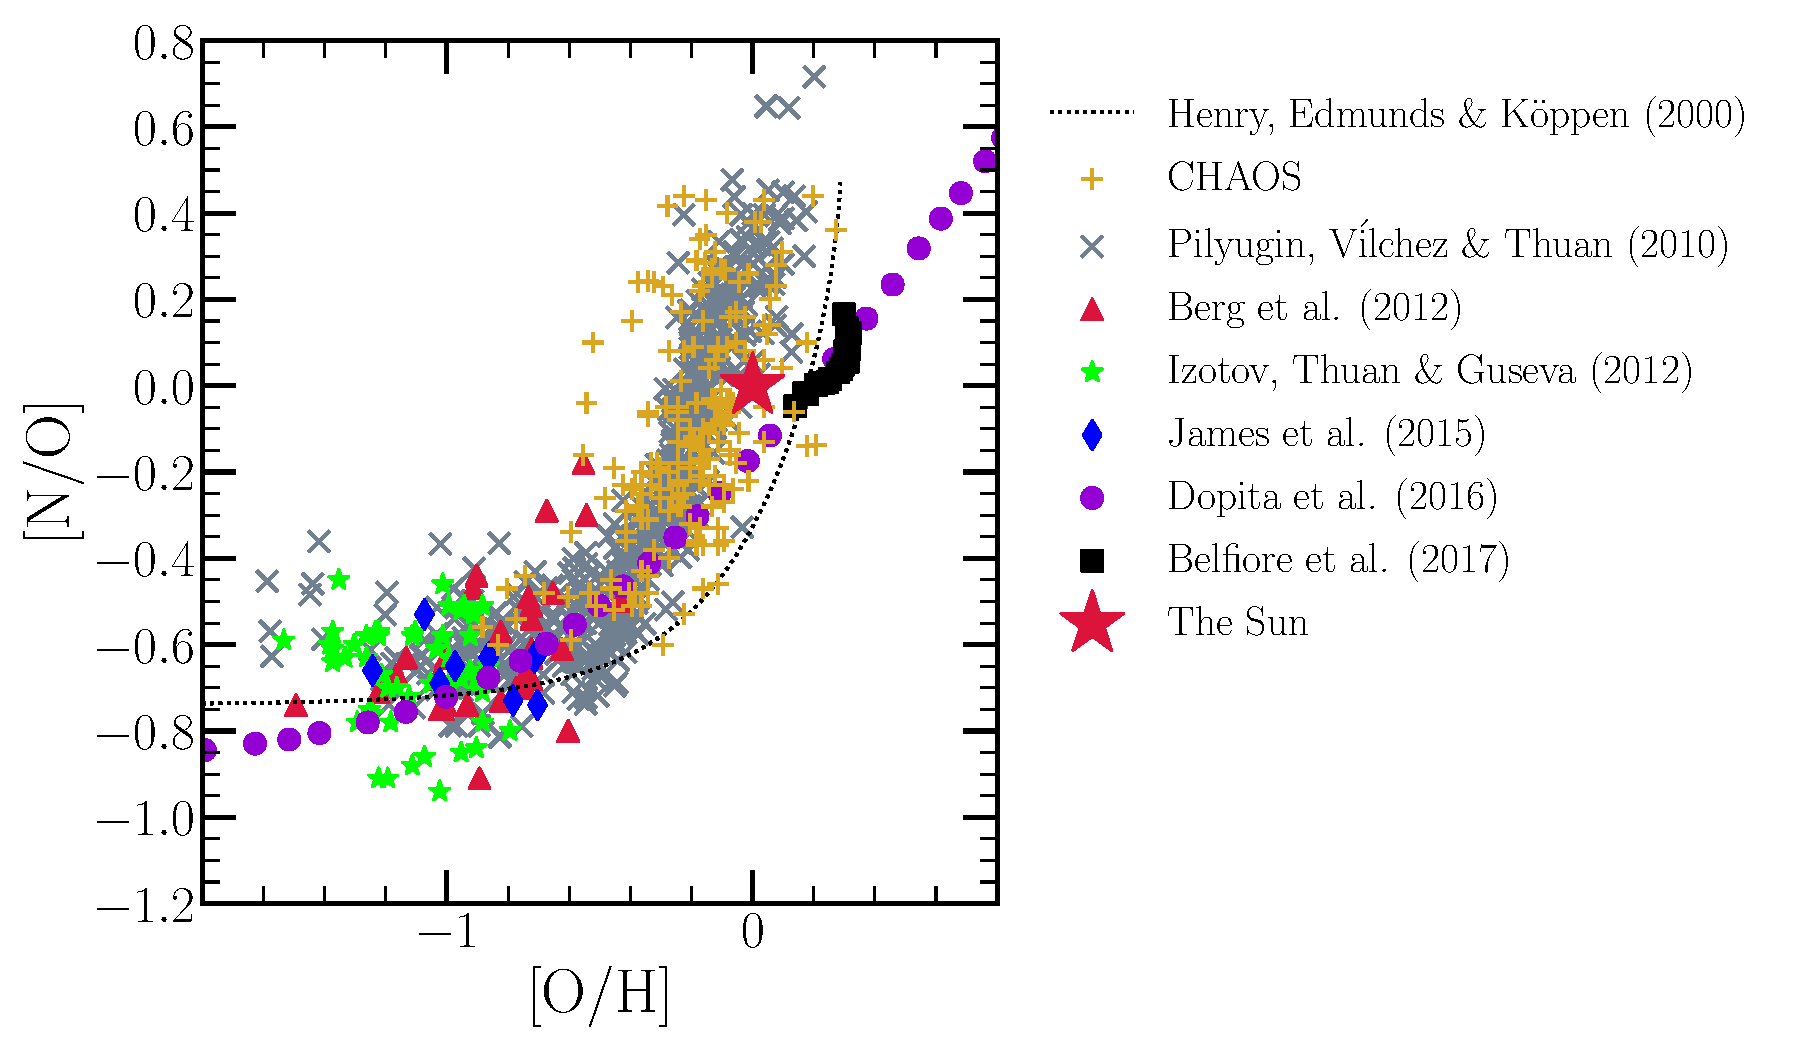
\includegraphics[scale = 0.63]{no_oh_observed.pdf}
\caption{
	The~\ohno~relation as observed in different galactic environments:
	HII regions from the first six CHAOS galaxies (golden +'s: NGC 3184, NGC
	628, NGC 5194, NGC 5457, M101, and NGC 2403;~\citealp{Berg2020,
	Skillman2020, Rogers2021}) and other nearby NGC spiral galaxies (grey X's;
	\citealp{Pilyugin2010}), HII regions in blue diffuse star forming dwarf
	galaxies (red triangles:~\citealp{Berg2012}; green stars:
	\citealp{Izotov2012}; blue diamonds:~\citealp{James2015}), in local stars
	and HII regions (purple circles:~\citealp{Dopita2016}), and in the MaNGA
	IFU survey (black squares:~\citealp{Belfiore2017}).
	The fit to~\no~as a function of~\oh~in Galactic and extragalactic HII
	regions by~\citet{Henry2000} is shown in a black dotted line.
	We omit all uncertainties for visual clarity.
	The Sun, at (0, 0) on this plot by definition, is marked by a large red
	star. 
}
\label{fig:no_oh_observed}
\end{figure*}

Observationally, N abundances are known to correlate strongly with O.
In Fig.~\ref{fig:no_oh_observed}, we present a compilation of such measurements:
\begin{enumerate}
	\item[\textbf{1.}] HII regions in the first six CHAOS\footnote{
		CHAOS: CHemical Abundances Of Spirals~\citep{Berg2015}
	} galaxies: NGC 3184, NGC 628, NGC 5194, NGC 5457, M101, and NGC 2403
	\citep{Berg2020, Skillman2020, Rogers2021}.

	\item[\textbf{2.}] HII regions in nearby NGC spirals~\citep*{Pilyugin2010}.

	\item[\textbf{3.}] HII regions in blue, diffuse star forming dwarf galaxies
	(\citealp{Berg2012};~\citealp*{Izotov2012};~\citealp{James2015}).

	\item[\textbf{4.}] Local stars and HII regions~\citep{Dopita2016}.

	\item[\textbf{5.}] Galactic and extragalactic HII regions
	\citep*{Henry2000}.

	\item[\textbf{6.}] Star-forming regions in 550  nearby galaxies in the
	MaNGA IFU\footnote{
		MaNGA: Mapping Nearby Galaxies at Apache Point Observatory
		\citep{Bundy2015}.
		IFU: Integral Field Unit.
	} survey~\citep{Belfiore2017}.
\end{enumerate}
Despite intrinsic scatter and some systematic variation in how the abundances
are determined, this~\ohno\footnote{
	We follow standard notation where [X/Y]
	$\equiv \log_{10}(X/Y) - \log_{10}(X/Y)_\odot$.
} relation is more or less the same across a wide range of astrophysical
environments.
Furthermore, recent arguments from both theoretical~\citep{Vincenzo2018} and
observational perspectives~\citep{HaydenPawson2021} suggest that this relation
is largely redshift-invariant.
Previous studies have interpreted this consistency as an indication that the
relation is nucleosynthetic in origin, reflective of a ``primary'' yield which
does not depend on a star's initial metal content and a ``secondary'' yield
which does (\citealp{VilaCostas1993};~\citealp*{vanZee1998};~\citealp{Henry1999,
PerezMontero2009};~\citealp*{Pilyugin2012};~\citealp{Andrews2013}).
Although we have highlighted star forming galaxies in
Fig.~\ref{fig:no_oh_observed}, N abundances are also easily measured in
massive ellipticals (see, e.g.,~\citealp{Schiavon2010},~\citealp{Conroy2013},
and~\citealp*{Conroy2014} for observational references), allowing it to
potentially bridge the gap between the physical processes affecting galaxies of
different morphologies.
\par
The largest source of uncertainty in understanding N abundances is that
accurate and precise nucleosynthetic yields from various enrichment channels
remain elusive.
Relative to other elements, N is a particularly difficult species to predict
yields for in stellar evolution models (see discussion in,
e.g.,~\citealp{Andrews2017}).
% No combination of models for massive star nucleosynthesis and their
% explodability is able to reproduce the observed abundance pattern of the
% elements, and N is no exception~\citep{Griffith2021a}.
In this paper, we constrain N yields empirically by testing the performance of
various assumptions within the framework of galactic chemical evolution (GCE)
models.
To this end we make use of the multi-zone model for the Milky Way published in
\citet{Johnson2021}, which treats the Galaxy as a series of concentric rings,
describing each one as a conventional one-zone model of chemical evolution
(see discussion in~\S~\ref{sec:multizone}).
This approach has been employed in the past to compute abundances for many
Galactic regions simultaneously (\citealp{Matteucci1989, Wyse1989, Prantzos1995,
Schoenrich2009};~\citealp*{Minchev2013, Minchev2014};~\citealp{Minchev2017};
\citealp*{Sharma2021}).
Because of the apparent universality of the~\ohno~relation, our results using
the Milky Way as a case test should apply to other galaxies as well.
\par
Recently,~\citet*{Grisoni2021} argued that rotating massive stars play a key
role in establishing the N abundances seen in metal-poor stars in the Milky Way.
Rotation has a considerable impact on the N yields of massive stars, because the
internal mixing that it causes~\citep{Zahn1992, Maeder1998, Lagarde2012} brings
internally produced C and O nuclei into the H-burning shell where they can be
processed into~\Nfourteen~via the CNO cycle~\citep{Heger2010, Frischknecht2016,
Andrews2017}.
We find similar results here comparing various theoretical models for
massive star nucleosynthesis (see discussion in~\S~\ref{sec:yields:ccsne}).
\par
Theoretical models for AGB star nucleosynthesis predict N yields to vary as a
function of progenitor mass and metallicity~\citep{Cristallo2011, Cristallo2015,
Karakas2010, Karakas2016, Karakas2018, Ventura2013, Ventura2014, Ventura2018,
Ventura2020}.
In sufficiently massive AGB stars, the base of the convective envelope is hot
enough to activate proton capture reactions, allowing the CNO cycle to convert
C and O isotopes in~\Nfourteen: a process known as hot bottom burning.
AGB stars are also known to experience thermal pulsations, and often these
pulations are accompanied by a penetration of the convective enevelope into the
CO-rich core, which incorporates some of this material into the envelope
itself: a process known as third dredge-up.
When both processes are active, third-dredge up adds new seed nuclei for hot
bottom burning to turn into~\Nfourteen, substantially increasing the N yields.
We demonstrate in~\S\S~\ref{sec:yields:agb} and~\ref{sec:yields:imf_agb} that
various theoretical models predict significantly different N yields for high
mass AGB stars as a consequence of how third dredge-up and hot bottom burning
occur in the models.
The differences in these processes are in turn a consequence of the uncertain
microphysical assumptions built into the stellar evolution models (e.g. mass
loss, opacity, convection and convective boundaries, nuclear reaction
networks).
In~\S~\ref{sec:results:yields}, we test the extent to which each of these
``off-the-shelf'' yield models are able to reproduce the~\ohno~relation in
GCE models.
\par
% In this paper, we aim to constrain N yields empirically by testing the
% performance of various ``off-the-shelf'' yield models within the framework of
% galactic chemical evolution (GCE) models.
% To this end we use the multi-zone model for the Milky Way published in
% \citet{Johnson2021}, which treats the Galaxy as a series of concentric rings,
% describing each ring as a conventional one-zone model of chemical evolution
% (see discussion in~\S~\ref{sec:multizone}).
% This approach has been employed in the past to compute abundance simultaneously
% for many Galactic regions (\citealp{Matteucci1989, Wyse1989, Prantzos1995,
% Schoenrich2009};~\citealp*{Minchev2013, Minchev2014};~\citealp{Minchev2017};
% \citealp*{Sharma2021}).
% In this paper, we assess what is required of N yields in order to reproduce
% various observed results, in particular the gas-phase~\ohno~relation
% illustrated in Fig.~\ref{fig:no_oh_observed}.
% Since a number of previous studies argue this result is nucleosynthetic in
% origin~\citep[e.g.][]{Pilyugin2012, Andrews2013}, our results from a GCE model
% for the Milky Way should apply to other systems as well.
% \par
In a sample of 6,507 galaxies from the MaNGA IFU survey~\citep{Bundy2015},
\citet{Schaefer2020} demonstrate that the intrinsic scatter in
the~\ohno~relation at fixed galaxy mass is correlated with variations in the
local star formation efficiency (SFE).
In regions of slower star formation,~\no~tends to be slightly higher at
fixed~\oh~(see their Fig. 4).
This is expected from simple GCE models, because more AGB stars enrich the
ISM with N by the time a given~\oh~is reached~\citep[e.g.][]{Molla2006,
Vincenzo2016a}.
However,~\citet{Schaefer2020} did not rule out stellar migration as an
additional source of scatter in the gas-phase~\ohno~relation.
In principle, there could be a deficit or surplus of N-producing AGB stars in a
given Galactic region at any time simply because the orbits are evolving,
driving additional scatter in the correlation.
The~\citet{Johnson2021} GCE model is the ideal tool with which to test this
hypothesis; the novel difference between theirs and previous models with
similar motivations is that it allows stellar populations to enrich
distributions of radii as they migrate.
Originally developed to study the abundances of O and iron (Fe), this aspect of
Galactic evolution turned out to have an important impact on the delayed type
Ia supernova (SN Ia) enrichment of Fe, causing complex fluctuations in the
enrichment rates with time at fixed radius.
Here we use the same methodology to test for similar effects in the delayed AGB
star production of N, in turn assessing whether migration or variability in the
SFE dominate scatter in the~\ohno~relation.
\par
With stellar abundance data, we can test the N abundances predicted by our
model against observables unavailable for the gas phase, such as age and~\ofe.
Using data from the Apache Point Observatory Galaxy Evolution Experiment
(APOGEE;~\citealp{Majewski2017}),~\citet{Vincenzo2021} demonstrate that when
stellar N abundances are corrected for internal mixing processes, the
correlations with stellar age and other elemental abundances are affected.
Whether or not our GCE model is able to reproduce their corrected data
constitutes a valuable test not only of our understanding of N nucleosynthesis,
but also the accuracy of the~\citet{Vincenzo2021} measurements which take a
model-dependent approach to estimate the birth abundances of N for APOGEE disc
stars with available age measurements.
\par
In~\S~\ref{sec:yields}, we discuss our adopted yields of N from its dominant
nucleosynthetic sources.
We discuss the details of our multi-zone chemical evolution model
in~\S~\ref{sec:multizone}.
We describe the evolution of a fiducial model in~\S~\ref{sec:results:fiducial}.
In~\S~\ref{sec:results:yields}, we quantify the~\ohno~relation predicted by our
model with various ``off-the-shelf'' AGB star yield models taken from the
literature.
We investigate the relative importance of the delay-time distribution and the
metallicity-dependence of AGB star yields in~\S~\ref{sec:results:t_z_dep_comp}.
We compare our model predictions to stellar N abundances corrected for internal
mixing processes in~\S~\ref{sec:results:vincenzo_comp}.
Lastly, we assess the sources of intrinsic scatter in the~\ohno~relation
in~\S~\ref{sec:results:schaefer_comp}.

\end{document}

